\documentclass[letterpaper,10pt,onecolumn]{article}
\usepackage[spanish]{babel}
\usepackage[utf8x]{inputenc}
\usepackage{amsfonts}
\usepackage{amsthm}
\usepackage{amsmath}
\usepackage{mathrsfs}
\usepackage{empheq}
\usepackage{enumitem}
\usepackage[pdftex]{color,graphicx}
\usepackage{hyperref}
\usepackage{listings}
\usepackage{calligra}
\usepackage{algpseudocode} 
\DeclareMathAlphabet{\mathcalligra}{T1}{calligra}{m}{n}
\DeclareFontShape{T1}{calligra}{m}{n}{<->s*[2.2]callig15}{}
\newcommand{\scripty}[1]{\ensuremath{\mathcalligra{#1}}}
\lstloadlanguages{[5.2]Mathematica}
\setlength{\oddsidemargin}{0cm}
\setlength{\textwidth}{490pt}
\setlength{\topmargin}{-40pt}
\addtolength{\hoffset}{-0.3cm}
\addtolength{\textheight}{4cm}

\begin{document}
\begin{center}



\includegraphics[width=490pt]{header.png}\\[0.5cm]

\textsc{\LARGE Taller 4 - F\'isica I (FISI-1018) - 2016-10}\\[0.5cm]

\textsc{\Large{Profesor: Jaime Forero}} \\[0.5cm]

\noindent\textsc{Ejercicios correspondiente a la clase complementaria de la semana del 15 de Febrero del 2016.}\\[0.5cm]
\end{center}

\noindent\textsc{Nota:} 
Los primeros tres ejercicios deben ser
entregados {\bf al comienzo} de la clase complementaria. Los \'ultimos
cuatro deben ser trabajados {\bf durante} la complementaria. 

La numeraci\'on
hace referencia al texto gu\'ia: \textit{F\'isica Universitaria Volumen
  1 (Sears-Semansky)}, decimotercera edici\'on, Pearson.

\begin{enumerate}
% aqui vienen los tres ejercicios "faciles"
\item Ejercicio 4.1 Angulo entre dos fuerzas.
\item Ejercicio 4.8  Viajando en un elevador.
\item Ejercicio 4.28  Dos bloques. %Juan Carlos

% aqui vienen los cuatro ejercicios "dificiles"
\item Problema 4.54 Dos bloques conectados por una cadena.

\item Un carro de masa $m$ se encuentra en una pendiente, cuyo ángulo de inclinación es $\theta$, y debido a una capa de hielo sobre la misma desliza sin fricción.
\begin{enumerate}
\item Calcule la aceleración del carro sobre la pendiente.
\item Suponga que la distancia desde el bumper delantero del carro hasta la base de la pendiente es $d$ y que el carro estaba parqueado antes de comenzar a deslizarse.¿cuánto tiempo tarda el carro en llegar a la base de la pendiente?, ¿con qué velocidad llega a dicho punto?
\end{enumerate}
\begin{figure}[hb]
\centering
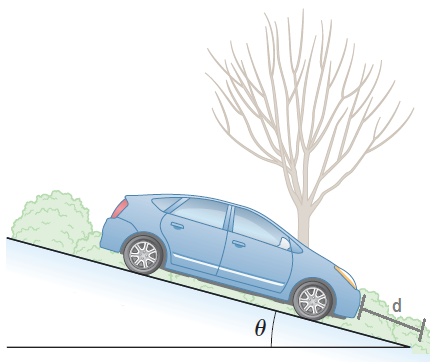
\includegraphics[width=0.5\textwidth]{carro.png}\\
\caption{Diagrama para el problema del carro}
\end{figure} %Juan Carlos

\item
Un atleta cuya masa es de $80kg$, está levantando pesas. Partiendo de una posición en reposo, levanta, con aceleración constante, una barra que pesa $320N$, elevándola $0.60m$ en $1.6s$. 
\begin{enumerate}
\item Dibuje un diagrama de cuerpo libre claramente especificado para la barra y para el atleta. 
\item
Use los diagramas del inciso anterior y las leyes de Newton para determinar la fuerza total que sus pies ejercen sobre el piso mientras levanta la barra.
\end{enumerate}
%Miguel

\item
Un automóvil entra a una curva de radio $R$, la carretera tiene un ángulo de inclinación $\theta$ y el coeficiente de fricción entre las llantas y el asfalto es $\mu$, ¿encuentre la máxima y mínima velocidad que puede tener el carro para mantenerse en la carretera sin deslizarse de lado?
Que pasa en el caso en que $\mu=1$ y $\theta=\pi/4$. 

\end{enumerate}

\end{document}

\begin{figure}[!h]
\begin{center}
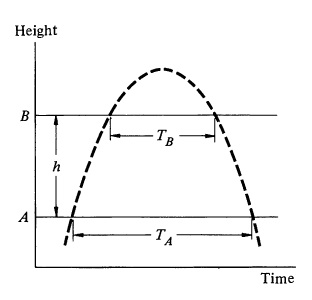
\includegraphics[scale=0.7]{altura.jpg} 
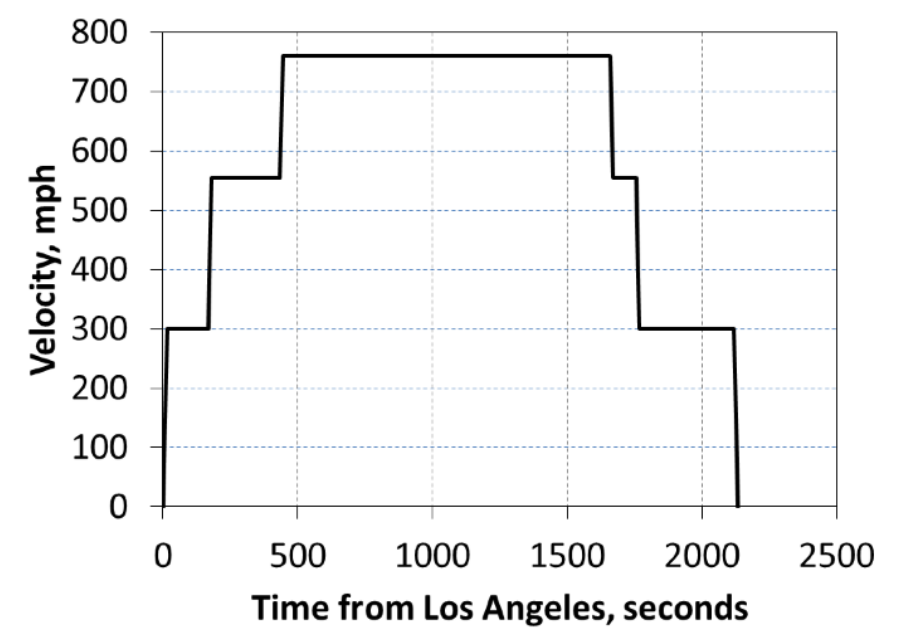
\includegraphics[scale=0.3]{hyperloop.png} 
\end{center}
\caption{Izquierda: diagrama para el ejercicio recomendado 3. Derecha: diagrama para el ejercicio recomendado 4.}
\label{fig:tiro}
\end{figure}





